\chapter{ПОДХОД МАШИННОГО ОБУЧЕНИЯ}

В этой главе будут даны основные определения, а также  сформулирована общая задача классификации.

Машинного обучение — это подраздел искусственного интелекта, находящийся на стыке статистики и компьютерных наук. Главная цель машинного обучения — создание методов, позволяющих строить математические модели и способных обучаться по прецедентам. Под обучением стоит понимать процесс аппроксимации заранее неизвестной функции по набору точек из её области определения и известных значений, полученных для каждой такой точки.

В нашем случае точки — это файлы формата .doc, а неизвестная функция отображает каждый такой файл во множество, состоящее из двух элементов {“вредоносный файл”, “безопасный файл”}.

Далее, мы более формально опишем, каким образом объекты  из реальной жизни можно рассматривать как точки, принадлежащие области определения неизвестной нам функции, и опишем подходы для извлечения зависимостей, c помощью которых в следующей главе будем решать задачи распознавания вредоносных программ.

\section{Обобщённая задача классификации}

Пусть $X$ — это множество объектов, а $Y$ — это множество классов.
Существует неизвестное нам отображение $F : X \to Y$, ставящее каждому объекту из $x \in X$ в соответствие метку класса из $y \in Y$.
Несмотря на то, что само отображение нам неизвестно, для некоторого набора элементов $\{ x_1, \dots , x_n \} \subset X$ мы можем получить значения $F$ в этих точках  $y_i = F(x_i)$ $i \subset \{ 1, \dots, n \}$.
В такой постановке задачи набор пар $\{ (x_1, y_1), \dots, (x_i, y_i) \}$ называется обучающей выборкой и, имея такую выборку, нам необходимо построить функцию $F^*$, которая наилучшим образом приближает функцию $F$.
Конечно, мы хотим чтобы построенная функция $F^*$ не только возвращала метку $y = F^*(x)$ для точки $x$ из обучающей выборки, но и могла возвращать метку для новых, ранее неизвестных нам объектов, руководствуясь некоторым правилом.

Поиск $F^*$ можно свести к минимизации некоторого функционала $M(F^*, F)$, отражающего близость $F^*$ к $F$. В качестве $M$ можно взять, например, квадрат разности, так называемый метод наименьших квадратов. Важно понимать, что уменьшение данной метрики на обучающей выборке не всегда приводит к уменьшению количества ошибок, совершаемых на новых объектах. Вопросы измерения качества классификации будут рассмотрены в следующих параграфах.

В некоторых случаях при использовании методов классификации нам важно знать не только конечную метку класса, но и степень уверенности в ней. В таком случае задачу классификации можно поставить следующим образом: существует неизвестное нам отображение $F : X \to Y$, ставящее каждому объекту из $X$ в соответствие метку класса из $Y$, необходимо по обучающей выборке $\{ (x_1, y_1), \dots, (x_i, y_i) \}$ получить функцию $F^* : X \to [0 \dots 1]^{|Y|}$, которая переводит объект в вектор вероятностей принадлежности к каждому из классов, и для любого $x \in X$ сумма $\sum_{i=1}^{|Y|} {F^*(x)}^{i} = 1$.

Получение значений приближенной функции $F^*$ предполагается производить на компьютере, поэтому алгоритм, который стоит за вычислением $F^*$, должен быть достаточно эффективным. 

Почти всегда функцию $F^*$ мы можем выбирать из некоторого параметризированного семейства функций, тогда задача поиска наилучшего приближения функции $F$ сводится к минимизации функционала $M(F^*, F)$ по вектору параметров, задающих $F^*$. Одним из подходов поиска параметров является градиентный спуск.

\section{Признаки объектов, матрица объект-признак}

Зачастую рассматриваемые нами объекты имеют довольно сложную структуру. Из-за этого могут появляться проблемы в формализации функций $F^*$ и $F$, введённых в предыдущем параграфе. Один из способов борьбы с такой проблемой — это перевод объекта в вектор формальных признаков.
Итак, пусть $x \in X$ — элемент множества $X$. Введём набор функций $D_i$, отображающие $x$ в признаки $d_i$.

Признаки могут быть различных типов, например:
\begin{itemize}
\item бинарный, $d_i \in \{0, 1\}$
\item категориальный, $d_i$ принадлежит конечному множеству несравнимых между собой элементов
\item количественный, $d_i \in R$
\end{itemize}

Имея $\{D_1,…,D_m\}$, мы можем построить для каждого из объектов $\{x_1,…,x_n\}$ их признаковое описание. Таким образом, вместо множества объектов произвольной структуры мы будем оперировать матрицей $D$ размера $n$ на $m$. Один из примеров такого подхода к решению задачи — это проблема классификации экземпляров цветка ириса. В этой проблеме для каждого объекта выделяются 4 количественных признака:

\begin{itemize}
\item длина чашелистика
\item ширина чашелистика
\item длина лепестка
\item ширина лепестка
\end{itemize}

В качестве классов представлены три вида ирисов:
\begin{itemize}
\item Iris setosa
\item Iris versicolor
\item Iris virginica 
\end{itemize}


\begin{table}[ht]
\caption{Фрагмент матрицы объект-признак задачи ирисов Фишера}
\label{tab_weight}
\centering
    \begin{tabular}{|c|c|c|c|c|}
    \hline Длина  & Ширина  & Длина  & Ширина  & Вид  \\
    чашелистика & чашелистика & лепестка & епестка & ириса \\
    \hline 5.1 & 3 & 1.4 & 0.2 & setosa  \\
    \hline 7 & 3.2 & 4.7 & 1.4 & versicolor  \\
    \hline 6.3 & 3.3 & 6 & 2.5 & virginica  \\
    \hline
    \end{tabular}
\end{table}

В дальнейшем, при решении задачи классификации вредоносных объектов мы также перейдём от файлов к их признаковым описаниям и впоследствии к матрице объект-признак.
Имея на руках такую матрицу, мы можем применять большинство методов машинного обучения.

\section{Линейные модели классификации}

Одним из самых простых и распространенных методов построения классификаторов является логистическая регрессия. Данный метод позволяет создавать модели предназначенные только для бинарной классификации. Без ограничения общности будем считать, что множество классов равно $\{0, 1\}$.

Для того, чтобы построить классификатор, нам нужна только матрица объект-признак, введенная ранее. Мы подаём её на вход, а на выход получаем линейную модель, задаваемую набором чисел $\{a_0, a_1,…, a_m\}$, где $m$ это количество признаков у объектов. 

После этапа обучения мы можем предсказывать класс новых объектов следующим образом. Пусть $x$ — это новый объект, используя ранее введёные функции $\{D_1, \dots, D_m \}$, создаём признаковое описание $\{d_1,…,d_m\}$ элемента $x$. На этом шаге важно использовать те же самые функции $D_i \in \{D_1, \dots, D_m \}$, с помощью которых была создана матрица объект-признак на этапе обучения.

Далее, мы вычисляем следующее выражение $ f \left( a_0 + \sum_{i=1}^{m} d_i * a_i \right)$, где $f \left( z \right) = \frac{1}{1 + e^{-z}}$. Значение данного выражения мы можем трактовать как вероятность принадлежности элемента к первому классу.

\begin{figure}[ht]
	\centering
    \begin{subfigure}[b]{1\textwidth}
    \centering
        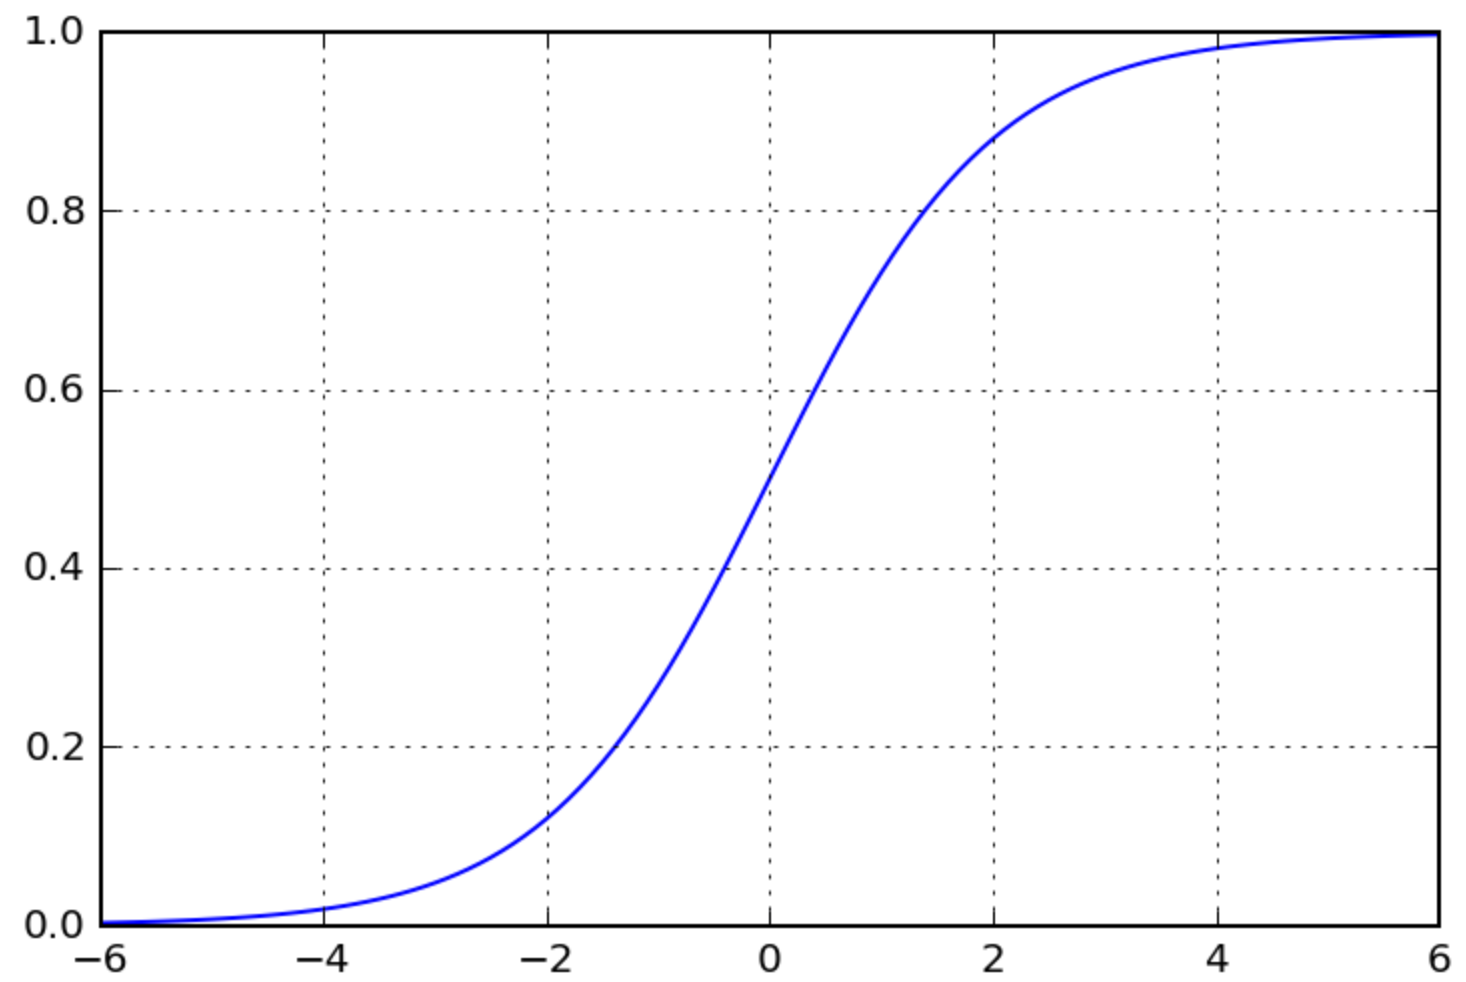
\includegraphics[scale=0.5]{pasted-image-15.png}
    \end{subfigure}
 
    \caption{График функции $f \left( z \right) = \frac{1}{1 + e^{-z}}$;}
    \label{fig_parsetree}
\end{figure}

Для поиска коэффициентов $\{a_0,…,a_m\}$, способствующих наилучшему приближению на обучающей выборке, существует множество эффективных методов. В дальнейшем мы будем использовать этот алгоритм для финального объединения результатов, полученных от большого набора других классификаторов. 

Данную модель можно интерпретировать следующим образом: модуль коэффициента при признаке под номером $i$ передаёт вес данного признака для итоговой оценки: чем он больше, тем важнее признак. Знак коэффициента отвечает за то, к какому классу мы будем отдавать предпочтение, если коэффициент отрицательный, то к классу “0”, если положительный, то, соответственно, классу “1”. Вычислив произведение вектора коэффициентов на вектор признаков, мы получаем число, которое необходимо сравнить с границей принятия решения $-a_0$. Если мы перешли эту границу, то метод будет отдавать предпочтение классу “1”, и, чем дальше данное число будет уходить за эту границу, тем больше вероятность принадлежности объекта к классу “1”. Конечно, данное рассуждение верно только для признаков, имеющих одиннаковый масштаб.

Конечно, логистическую регрессию можно использовать не только как способ объеденения других классификаторов. Ниже я привожу пример решения задачи классификации цветков ириса. Для возможности визуалиации  я предварительно понизил размерность вектора признаков каждого объекта с четырёх признаков до двух. Для понижения размерности я воспользовался методом главных компонент \cite{pca_book}\cite{pca_program}.

\begin{figure}[ht]
	\centering
    \begin{subfigure}[b]{1\textwidth}
    \centering
        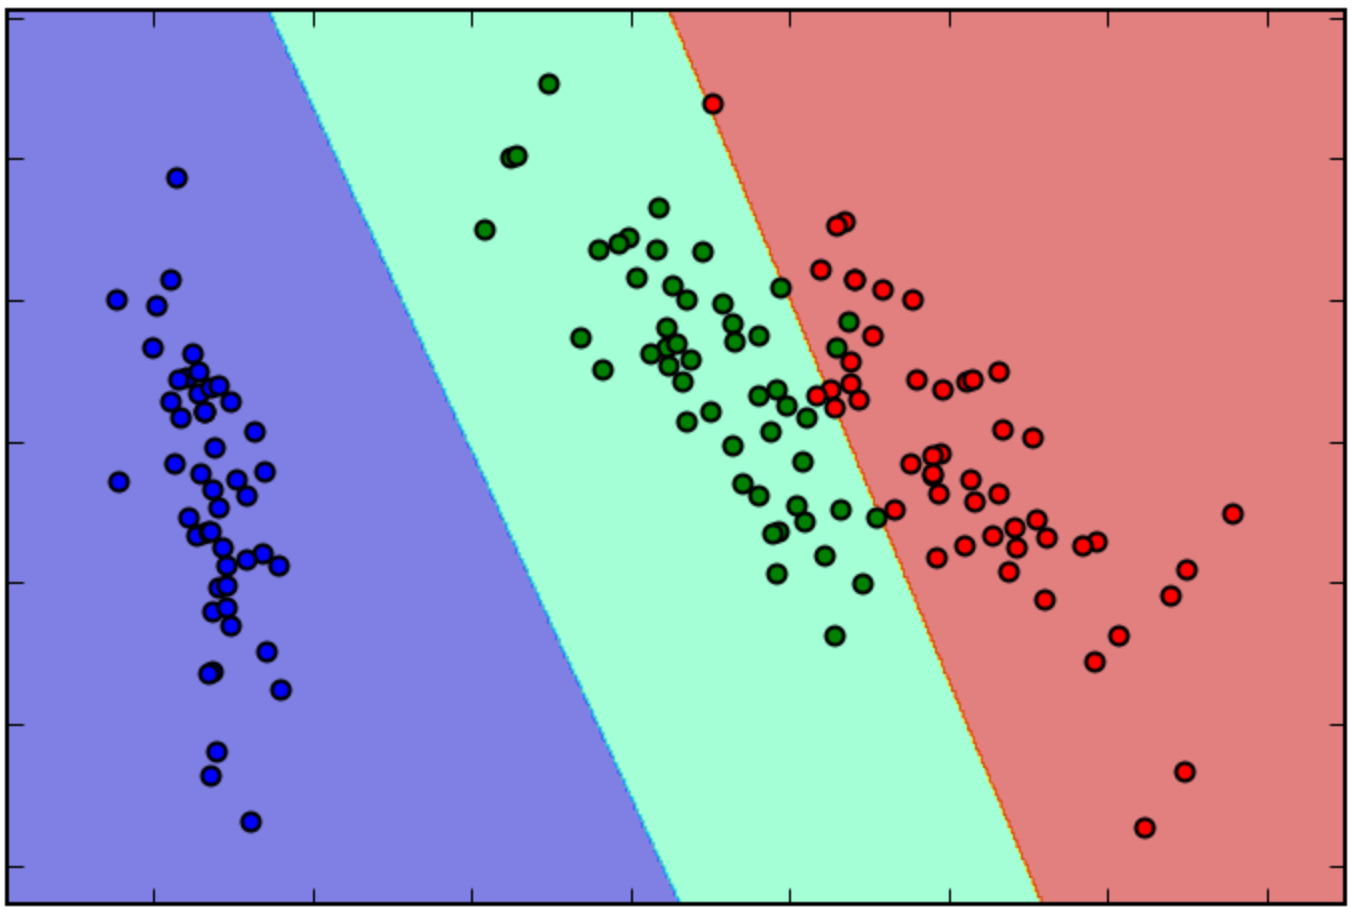
\includegraphics[scale=0.5]{pasted-image-19.png}        
    \end{subfigure}
 
    \caption{Ирисы Фишера, границы классов, полученные методом логистической регрессии;}
    \label{fig_parsetree}
\end{figure}
